%% abtex2-modelo-trabalho-academico.tex, v-1.9.5 laurocesar
%% Copyright 2012-2015 by abnTeX2 group at http://www.abntex.net.br/ 
%%
%% This work may be distributed and/or modified under the
%% conditions of the LaTeX Project Public License, either version 1.3
%% of this license or (at your option) any later version.
%% The latest version of this license is in
%%   http://www.latex-project.org/lppl.txt
%% and version 1.3 or later is part of all distributions of LaTeX
%% version 2005/12/01 or later.
%%
%% This work has the LPPL maintenance status `maintained'.
%% 
%% The Current Maintainer of this work is the abnTeX2 team, led
%% by Lauro César Araujo. Further information are available on 
%% http://www.abntex.net.br/
%%
%% This work consists of the files abntex2-modelo-trabalho-academico.tex,
%% abntex2-modelo-include-comandos and abntex2-modelo-references.bib
%%

% ------------------------------------------------------------------------
% ------------------------------------------------------------------------
% abnTeX2: Modelo de Trabalho Academico (tese de doutorado, dissertacao de
% mestrado e trabalhos monograficos em geral) em conformidade com 
% ABNT NBR 14724:2011: Informacao e documentacao - Trabalhos academicos -
% Apresentacao
% ------------------------------------------------------------------------
% ------------------------------------------------------------------------

\documentclass[
	% -- opções da classe memoir --
	12pt,				% tamanho da fonte
	openright,			% capítulos começam em pág ímpar (insere página vazia caso preciso)
	oneside,			% para impressão apenas no verso. Oposto a twoside
	% twoside,			% para impressão em verso e anverso. Oposto a oneside
	a4paper,			% tamanho do papel. 
	% -- opções da classe abntex2 --
	%chapter=TITLE,		% títulos de capítulos convertidos em letras maiúsculas
	%section=TITLE,		% títulos de seções convertidos em letras maiúsculas
	%subsection=TITLE,	% títulos de subseções convertidos em letras maiúsculas
	%subsubsection=TITLE,% títulos de subsubseções convertidos em letras maiúsculas
	% -- opções do pacote babel --
	english,			% idioma adicional para hifenização
	french,				% idioma adicional para hifenização
	spanish,			% idioma adicional para hifenização
	brazil				% o último idioma é o principal do documento
]{abntex2}

% ---
% Pacotes básicos 
% ---
\usepackage{lmodern}			% Usa a fonte Latin Modern			
\usepackage[T1]{fontenc}		% Selecao de codigos de fonte.
\usepackage[utf8]{inputenc}		% Codificacao do documento (conversão automática dos acentos)
\usepackage{lastpage}			% Usado pela Ficha catalográfica
\usepackage{indentfirst}		% Indenta o primeiro parágrafo de cada seção.
\usepackage{color}				% Controle das cores
\usepackage{graphicx}			% Inclusão de gráficos
\usepackage{microtype} 			% para melhorias de justificação
\usepackage{booktabs}
\usepackage{graphicx}
\usepackage[table,xcdraw]{xcolor}
\usepackage{float}
% ---

% ---
% Pacotes adicionais, usados apenas no âmbito do Modelo Canônico do abnteX2
% ---
\usepackage{lipsum}				% para geração de dummy text
% ---

% ---
% Pacotes de citações
% ---
\usepackage[brazilian,hyperpageref]{backref}	 % Paginas com as citações na bibl
\usepackage[alf]{abntex2cite}	% Citações padrão ABNT

% --- 
% CONFIGURAÇÕES DE PACOTES
% --- 

% ---
% Configurações do pacote backref
% Usado sem a opção hyperpageref de backref
\renewcommand{\backrefpagesname}{Citado na (s) página (s):~} % Texto padrão antes do número das páginas

\renewcommand{\backref}{}
% Define os textos da citação
\renewcommand*{\backrefalt}[4]{
	\ifcase#1
		Nenhuma citação no texto.%
	\or{}
		Citado na página #2.%
	\else
		Citado #1 vezes nas páginas #2.%
	\fi}%
% ---
\setlength{\parindent}{1.3cm} % --- Espaçamentos entre linhas e parágrafos --- % 
\setlength{\parskip}{0.2cm}  % Controle do espaçamento entre um parágrafo e outro: tente também \onelineskip
% Seleciona o idioma do documento (conforme pacotes do babel)
%\selectlanguage{english}
\selectlanguage{brazil}
\frenchspacing % Retira espaço extra obsoleto entre as frases.
\makeindex % --- compila o indice --- %

% --- Informações de dados para CAPA e FOLHA DE ROSTO --- %

\autor{João Vítor Fernandes Dias}
\titulo{\textit{Timetabling Problem}: desafios no desenvolvimento de um sistema de decisão voltado ao problema de organização de grade horária do ensino superior}
\local{Campos dos Goytacazes, RJ}
\data{\today}

\def\orientadorTCC{FermÍn Alfredo Tang Montané}

\preambulo{Trabalho de Conclusão de Curso apresentado ao Curso de Graduação em Ciência da Computação da Universidade Estadual do Norte Fluminense Darcy Ribeiro, sob orientação do Prof. Dr. \orientadorTCC}
% \instituicao{Universidade Estadual do Norte Fluminense Darcy Ribeiro \par Ciência da Computação \par Metodologia de Pesquisa}
\orientador{\orientadorTCC}
\tipotrabalho{Projeto de Pesquisa}
%\coorientador{Equipe \abnTeX}
% O preambulo deve conter o tipo do trabalho, o objetivo, o nome da instituição e a área de concentração
% ---

% ---
% Configurações de aparência do PDF final
% alterando o aspecto da cor azul
\definecolor{blue}{RGB}{41,5,195}

% informações do PDF
\makeatletter
\hypersetup{
%pagebackref=true,
    pdftitle={\@title}, 
    pdfauthor={\@author},
    pdfsubject={\imprimirpreambulo},
    pdfcreator={LaTeX with abnTeX2},
    pdfkeywords={abnt}{latex}{abntex}{abntex2}{trabalho acadêmico}, 
    colorlinks=true,       		% false: boxed links; true: colored links
    linkcolor=blue,          	% color of internal links
    citecolor=blue,        		% color of links to bibliography
    filecolor=magenta,      		% color of file links
    urlcolor=blue,
    bookmarksdepth=4
}
\makeatother

\begin{document} % --- Início do documento --- %

\pretextual                 % --- INÍCIO DOS ELEMENTOS PRÉ-TEXTUAIS --- %

    \imprimircapa           % Capa
    \imprimirfolhaderosto   % Folha de rosto (o * indica que haverá a ficha bibliográfica)
    
    % % ---
% Inserir a ficha bibliografica
% ---

% Isto é um exemplo de Ficha Catalográfica, ou ``Dados internacionais de
% catalogação-na-publicação''. Você pode utilizar este modelo como referência. 
% Porém, provavelmente a biblioteca da sua universidade lhe fornecerá um PDF
% com a ficha catalográfica definitiva após a defesa do trabalho. Quando estiver
% com o documento, salve-o como PDF no diretório do seu projeto e substitua todo
% o conteúdo de implementação deste arquivo pelo comando abaixo:
%
% \begin{fichacatalografica}
%     \includepdf{fig_ficha_catalografica.pdf}
% \end{fichacatalografica}

\begin{fichacatalografica}
    \sffamily
    \vspace*{\fill}					% Posição vertical
    \begin{center}					% Minipage Centralizado
    \fbox{\begin{minipage}[c][8cm]{13.5cm}		% Largura
    \small
    \imprimirautor
    %Sobrenome, Nome do autor
    
    \hspace{0.5cm} \imprimirtitulo  / \imprimirautor. --
    \imprimirlocal, \imprimirdata-
    
    \hspace{0.5cm} \pageref{LastPage} p. : il. \\ % (algumas color.) ; 30 cm.\\
    
    \hspace{0.5cm} \imprimirorientadorRotulo~\imprimirorientador\\
    
    \hspace{0.5cm}
    \parbox[t]{\textwidth}{\imprimirtipotrabalho~--~\imprimirinstituicao,
    \imprimirdata.}\\
    
    \hspace{0.5cm}
    1. Veículos autônomos. 
    2. Inteligência Artificial.
    3. Machine Learning.
    4. Condução Autônoma.
    I. Manuel Antonio Molina Palma.
    II. Universidade Estadual do Norte Fluminense Darcy Ribeiro.
    III. Faculdade de Ciência da Computação.
    IV. Veículos autônomos e inteligência artificial:
    um estudo sobre a implementação no brasil.
    \end{minipage}}
    \end{center}
    \end{fichacatalografica}   % --- FICHA CATALOGRÁFICA --- % NÃO DEVE SER USADO
    % % Sim, tá vazio.                % --- ERRATA --- % NÃO HÁ ERRATA
    % % Inserir folha de aprovação
% ---

% Isto é um exemplo de Folha de aprovação, elemento obrigatório da NBR
% 14724/2011 (seção 4.2.1.3). Você pode utilizar este modelo até a aprovação
% do trabalho. Após isso, substitua todo o conteúdo deste arquivo por uma
% imagem da página assinada pela banca com o comando abaixo:
%
% \includepdf{folhadeaprovacao_final.pdf}
%
\begin{folhadeaprovacao}

    \begin{center}
    {\ABNTEXchapterfont\large\imprimirautor}
    
    \vspace*{\fill}\vspace*{\fill}
    \begin{center}
    \ABNTEXchapterfont\bfseries\Large\imprimirtitulo
    \end{center}
    \vspace*{\fill}
    
    \hspace{.45\textwidth}
    \begin{minipage}{.5\textwidth}
    \imprimirpreambulo
    \end{minipage}%
    \vspace*{\fill}
    \end{center}
    
    Trabalho aprovado. \imprimirlocal, 22 de Junho de 2022:
    
    \assinatura{\textbf{\imprimirorientador} \\ Orientador} 
    %\assinatura{\textbf{Professor} \\ Convidado 1}
    % \assinatura{\textbf{Professor} \\ Convidado 2}
    %\assinatura{\textbf{Professor} \\ Convidado 3}
    %\assinatura{\textbf{Professor} \\ Convidado 4}
    
    \begin{center}
    \vspace*{0.5cm}
    {\large\imprimirlocal}
    \par
    {\large\imprimirdata}
    \vspace*{1cm}
    \end{center}
    
    \end{folhadeaprovacao}    % --- FOLHA DE APROVAÇÃO --- % REALMENTE NECESSÁRIO?
    % \begin{dedicatoria}
   \vspace*{\fill}
   \centering
   \noindent
   \textit{ Este trabalho é dedicado às crianças adultas que,\\
   quando pequenas, sonharam em se tornar cientistas.} \vspace*{\fill}
\end{dedicatoria}           % --- DEDICATÓRIA --- % REALMENTE NECESSÁRIO?
    % \begin{agradecimentos}
Agradeço aos meus pais que se dedicaram para que eu pudesse estar cursando esta graduação, assim podendo completar mais uma etapa da minha vida. 
Sem o apoio, conselhos, carinho e amor, nada disso seria possível. Sou eternamente grato por tudo que vocês fazem e sempre fizeram para que minha vida fosse especial. 

Agradeço ao professor Dr. Manuel Antonio Molina Palma pela dedicação e paciência durante o lecionamento desta disciplina, e obrigado pela ajuda e por estar disponível nos momentos de necessidade.   

Por último, mas não menos importante, agradeço a toda minha família e amigos que estiveram comigo em todos os momentos da minha vida.
\end{agradecimentos}        % --- AGRADECIMENTOS --- % REALMENTE NECESSÁRIO?
    % \begin{epigrafe}
    \vspace*{\fill}
	\begin{flushright}
		\textit{``Behind me lies a farm. \\
		I wonder if there is bread above the hearth \\
		and if I will ever return. \\
		(Pantheon, League of Legends)}
	\end{flushright}
\end{epigrafe}              % --- EPÍGRAFE --- % REALMENTE NECESSÁRIO?
    \pdfbookmark[0]{\listfigurename}{lof}
\listoffigures*
\cleardoublepage            % --- inserir lista de ilustrações --- % NÃO USADO
    % \begin{siglas}
  \item[PDTU] Plano Diretor de Transporte Urbano
  \item[ML] Machine Learning 
  \item[IA] Inteligência Artificial
\end{siglas}               % --- inserir lista de abreviaturas e siglas --- % NÃO USADO
                                                % --- inserir lista de símbolos --- % NÃO USADO
                                                % --- inserir o sumario --- %
    
    % % resumo em português
\setlength{\absparsep}{18pt} % ajusta o espaçamento dos parágrafos do resumo
\begin{resumo}

    Este artigo visa apresentar uma análise da situação em que atualmente se encontra a criação de grades horárias na Universidade Estadual do Norte Fluminense, bem como apontar seus maiores problemas e desenvolver um sistema de decisão capaz de auxiliar diversos centros e laboratórios no desenvolvimento de suas grades horárias, buscando a otimização do uso de salas e redução dos conflitos existentes entre demandas de diferentes alunos por matérias.
    
    \textbf{Palavras-chave}: Tabela de horários, Agendamento de aulas universitárias, Heurísticas, Programação Inteira, Representação do Conhecimento, Interação Homem Computador.

\end{resumo}
                % --- RESUMOS --- %
    % % resumo em inglês
\begin{resumo}[Abstract]
    \begin{otherlanguage*}{english}

        This paper aims to present an analysis of the current situation of the schedule creation at the Universidade Estadual do Norte Fluminense, as well as to point out its major problems and to develop a decision system capable of helping several centers and laboratories in the development of their schedules, seeking to optimize the use of rooms and to reduce the conflicts between different students' demands for subjects.
        
        \vspace{\onelineskip}
        
        % \noindent
        \textbf{Keywords}: Timetabling, University class scheduling, Heuristics, Integer Programming, Knowledge Representation, Human Computer Interaction.

    \end{otherlanguage*}
\end{resumo}              % --- ABSTRACT --- %
    % \pdfbookmark[0]{\listtablename}{lot}
\listoftables*
\cleardoublepage                % --- inserir lista de tabelas --- %
    \pdfbookmark[0]{\contentsname}{toc}
\tableofcontents*
\cleardoublepage

\textual                                        % --- INÍCIO DOS ELEMENTOS TEXTUAIS --- %
    
    % --- Introdução --- % (exemplo de capítulo sem numeração, mas presente no Sumário)

\chapter[Introdução]{Introdução}
% \addcontentsline{toc}{chapter}{Introdução}

% ----------------------------------------------------------

Na realidade do ensino superior brasileiro, mas não limitado a ele, nem todos estudantes são aprovados em todas as disciplinas que escolheram cursar em determinado semestre. Assim, causando um atrito na possível simetria na demanda dos alunos por matérias ao longo dos semestres. Além desta questão, surge também a decisão dos coordenadores de curso quanto a qual professor será associado a qual disciplina, bem como, quais serão essas disciplinas e em qual sala devem ser alocadas.

Dada grande quantidade de variáveis interconectadas e as características específicas de cada instituição \cite{MIRANDA2012505}, a organização destas informações buscando a melhor solução possível apresenta-se como um desafio. Principalmente se considerarmos que esta solução é buscada manualmente, estando também passível de erros humanos.

Embora seja um problema atual, isso não significa que seja recente. Desde 1978 \cite{BARHAM1978} o termo \textit{timetabling} encontra-se no meio acadêmico como o termo referente ao tabelamento de grade horária, sendo assim, é este o termo que será principalmente utilizado neste trabalho. Neste artigo de 1978 já se propunha uma forma para que se obtivesse um tabelamento otimizado, e demonstrava que o método utilizado gerava bons resultados.
    \chapter{Contexto acadêmico do \textit{Timetabling Problem}} % ## 2. Contexto do *Timetabling Problem* no meio acadêmico

Antes de prosseguirmos com o desenrolar deste trabalho, é adequado que primeiro definamos alguns parâmetros para o melhor entendimento do que está por vir.

\section{Definição de termos} % ### 2.1 Definição de termos

Ao longo dos anos de desenvolvimento acadêmico, diversos assuntos vão se aprofundando e se tornando mais específicos, assim, os estudiosos acabam cunhando novos termos que o auxiliam a desvencilhar as novas áreas específicas das suas áreas originárias. Porém, existe o potencial de que haja um crescimento desestruturado destes novos termos, assim vários termos diferentes podem se referir a um mesmo conceito, enquanto que um mesmo tempo pode se referir a vários conceitos diferentes de acordo com o autor.

Assim como feito por \cite{goos_scheduling_1996}, definiremos os conceitos dos termos que serão usados ao longo deste trabalho.

O termo "\textit{timetable}" tem o mesmo valor que "grade horária" e serão usadas como se fossem sinônimos mesmo sendo de línguas diferentes. Segundo \cite{goos_scheduling_1996}, podemos definir \textit{timetable} como uma estrutura que mostra quando que eventos ocorrerão, não havendo necessariamente a alocação de recursos.

Vale ressaltar que este termo não tem seu uso limitado para os fins desta pesquisa, sendo também usado para problemas de alocação de enfermeiros, esportes, funcionários e transportes \cite{arratia-martinez_university_2021}. Entretanto, neste trabalho, abordaremos principalmente os termos relacionados ao que pode ser chamado de \textit{Educational Timetabling} (Ed-TT) \cite{alencar_visualization_2019}, que é o que tende a envolver um conjunto específico de recursos relacionados à educação.

Wren também define os conceitos para \textit{class timetable}, \textit{university examination timetable} e \textit{university class timetable}, tendo relevância apenas o último, que considera a disponibilidade de professores e salas, a quantidade de alunos e os requisitos que determinada disciplina exige.

Exemplo: Enquanto que a disciplina "Laboratório de Física" exige que a aula seja ministrada em um tipo de sala específica com os equipamentos necessários, a disciplina "computação e sociedade" não apresenta esta restrição, ficando limitada apenas à quantidade de pessoas na turma.

Aqui, visto que uma solução final envolverá várias dimensões (Professores x Disciplinas x Sala x Alunos x Horários x Dias), consideraremos \textit{timetable} como esse pacote de valores distribuídos em uma só estrutura. Para que esses valores sejam distribuídos, daremos o nome de \textbf{alocação} ao ato de criar qualquer relação entre as dimensões. Como a relação de horários e dias será considerada fixa, a \textbf{alocação} se referirá à atribuição como a de professores a disciplinas, disciplinas a salas, disciplinas a um determinado padrão de dias e horários, etc.

Para que esta alocação ocorra, é necessário atender a certos critérios, e aí entra o "problema de organização de grade horária", também chamado de \textit{timetabling problem}. Esta é uma subcategoria do \textbf{problema de agendamento} (\textit{scheduling Optimization Problem}) \cite{alencar_visualization_2019} que por sua vez é definido por \cite{goos_scheduling_1996} como sendo:

\begin{quote}\footnotesize
    Resolver problemas práticos relacionados à alocação, sujeito a restrições, de recursos a objetos sendo colocados no espaço-tempo, usando ou desenvolvendo quaisquer ferramentas que possam ser apropriadas. Os problemas irão frequentemente se relacionar à satisfação de certos objetivos.
\end{quote}

Outro termo relevante a se pontuar são as \textit{hard and soft constraints} que podemos chamar de restrições rígidas e flexíveis. \cite{alencar_visualization_2019} as define dizendo que as restrições rígidas são de atendimento obrigatório, enquanto as restrições flexíveis são opcionais, mas convenientes para melhorar a qualidade da solução obtida.

Exemplo de restrição rígida: nem professores nem alunos podem ser alocados simultaneamente a duas salas ou disciplinas simultaneamente. Uma solução que viole esta restrição se torna automaticamente inviável.

Exemplo de restrição flexível: professor J. prefere não dar aulas nas tardes de sexta-feira, e prefere dar aula nas manhãs da segunda-feira. Uma solução que viole esta restrição não se torna inviável, porém tende a ter menos valor neste critério do que uma solução que siga as preferências definidas.

Alguns outros termos similares a este campo de pesquisa encontrados na literatura são \textit{periodic event scheduling problem}, \textit{timetable scheduling}, \textit{class scheduling}, \textit{student scheduling}, \textit{university course timetabling}, dentre outros.

\section{Métodos de resolução} % ### 2.2. Métodos de resolução

% <!--
% - O problema de timetabling   a
%   - Origem                    a
%   - Repartições               a
%   - Escopo maior              a
%     - Scheduling              a
%   - Escopo menor              a
%     - Exam                    a
%     - Class                   a
% - TT
%   - Soluções
%   - Desafios
%   - Diversas formas de resolução
%     - Graph Coloring
%     - Heurísticas
%     - Meta-heurísticas
%     - IA
%     - etc.
% - Visualização de informações
%   - Benefícios
%   - Motivações
%   - Relação com timetabling
% - Problema geral a ser resolvido
%   - Multi dimensionalidade
%     - Professores
%     - Alunos
%     - Salas
%     - Departamentos
%       - Preferências
%       - Concorrências
%   - Otimalidade
%   - Erros humanos
%   - Número de possibilidades
%   - Interface intuitiva e relevante é um desafio com poucos estudos nos últimos anos
% - Problemas específicos
%   - Regras específicas
%   - Prioridades diferentes
%   - estrutura organizacional semi-exclusiva
% -->

% <!-- Pesquisar posteriormente sobre imagens que ilustrem bem as diferentes sub categorias de scheduling -->

Existem diversas implementações já realizadas, utilizando uma miríade de métodos. Em seu trabalho \cite{miranda_udpskeduler_2012}, J. Miranda informa sobre diversos sistemas baseados em computador para auxiliar na tarefa de agendamento. J. Miranda também cita um dos métodos de resolução como sendo o \textbf{modelo de programação inteira} e \textbf{heurísticas}.

Outros trabalhos buscaram condensar em forma de tabela as informações encontradas. Abaixo estão dispostas algumas das tabelas encontradas durante o estudo bibliográfico e que foram elaboradas por diversos autores.

Na figura \ref{Desenvolvimento}, \cite{alegre_desenvolvimento_2012} traça a relação entre os diversos autores, ano de sua publicação e seu país de origem com os dados encontrados em seus trabalhos quanto aos parâmetros utilizados na elaboração da grade horária, quão grandes eram cada um de seus parâmetros, quanto tempo foi necessário para achar uma solução e quais foram as técnicas utilizadas.

% Entender o que tá dando errado aqui depois

\begin{figure}[htbp]\centering
    \caption{\label{Desenvolvimento}Resumo de trabalhos, parâmetros, dimensões, tempo e técnicas.}
    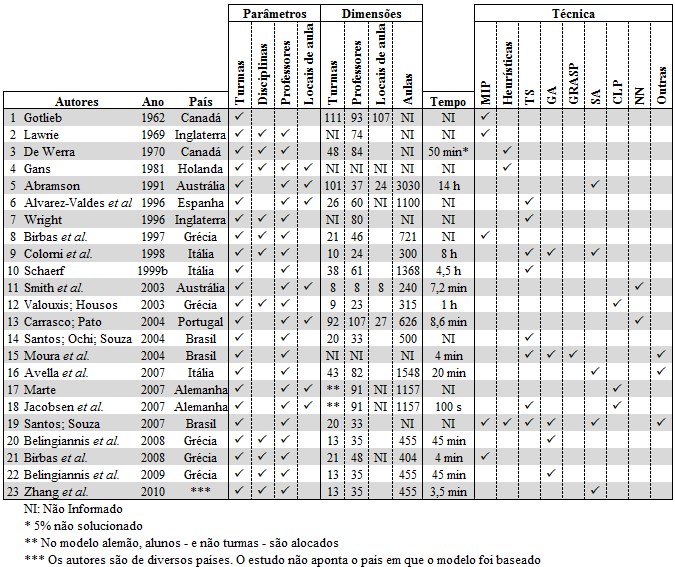
\includegraphics[angle=0,scale=1]{files/img/tabelas/Desenvolvimento.png}
    \legend{Fonte: \cite{alegre_desenvolvimento_2012}}
\end{figure}    % Desenvolvimento

Na figura \ref{University}, \cite{arratia-martinez_university_2021}, apresenta uma comparação similar à anterior, porém não separada em categorias, apenas categorizando entre verdadeiro e falso algumas características como alocação de salas, professores, nível institucional e método exato ou inexato.

\begin{figure}[htbp]\centering
    \caption{\label{University}Comparação entre artigos que solucionam o problema de grade horária}
    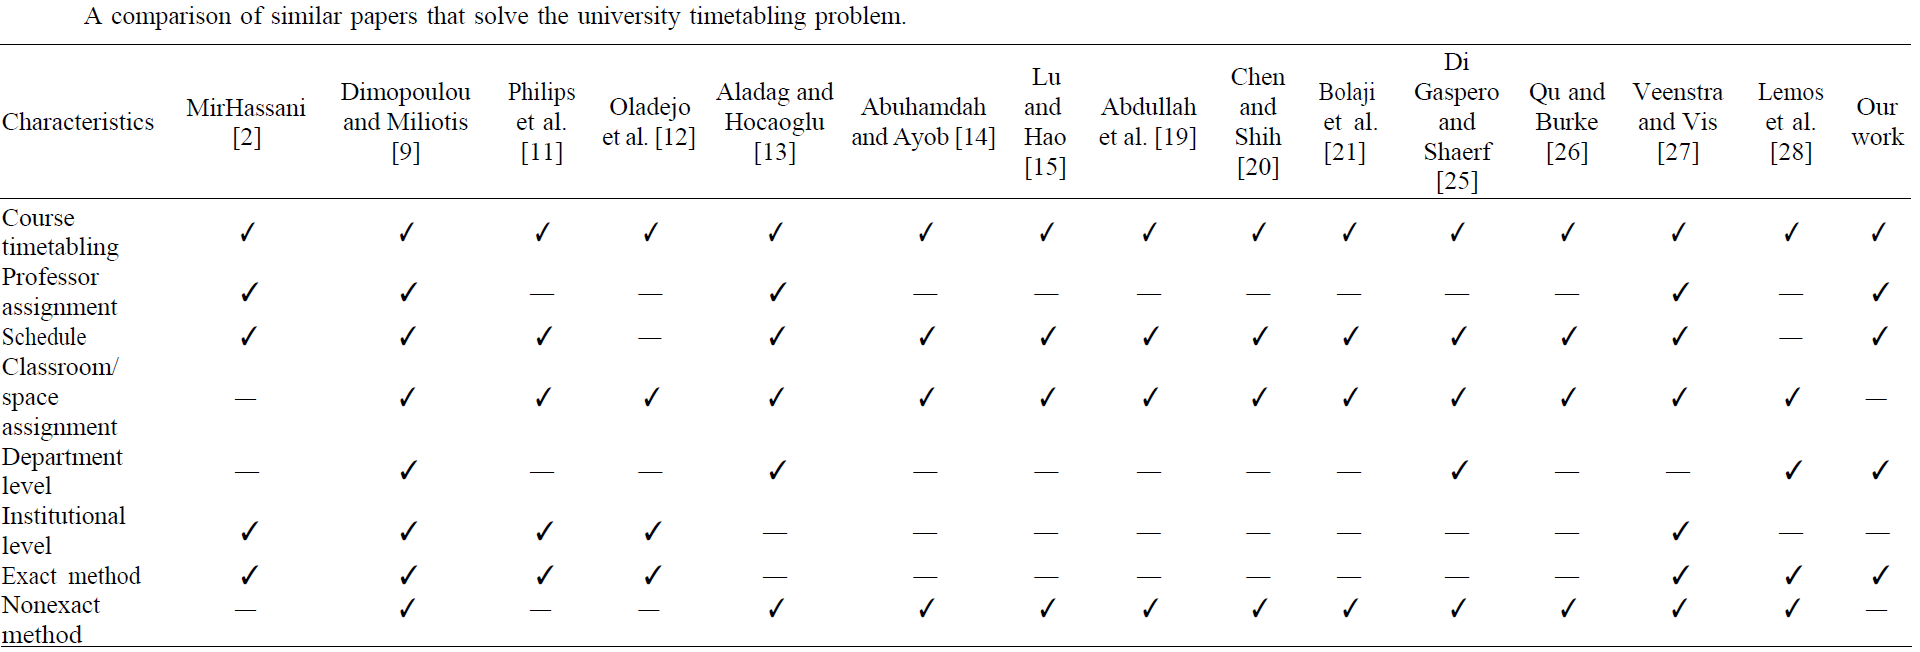
\includegraphics[angle=0,scale=0.37]{files/img/tabelas/University.png}
    \legend{Fonte: \cite{arratia-martinez_university_2021} - editado}
\end{figure}    % University

Na figura \ref{Visualization}, \cite{alencar_visualization_2019} explora uma categoria mais específica do problema, que é a característica da interatividade das interfaces desenvolvidas. Este apresenta características qualitativas quanto aos métodos, os dados dispostos, as técnicas de interação e o método utilizado para solucionar o problema de grade horária educacional. Nesta figura, os autores usam "Y" para simbolizar "Sim", "N" para "Não" e "-" para "Inconclusivo".

\begin{figure}[htbp]\centering
    \caption{\label{Visualization}Análise de publicações aceitas.}
    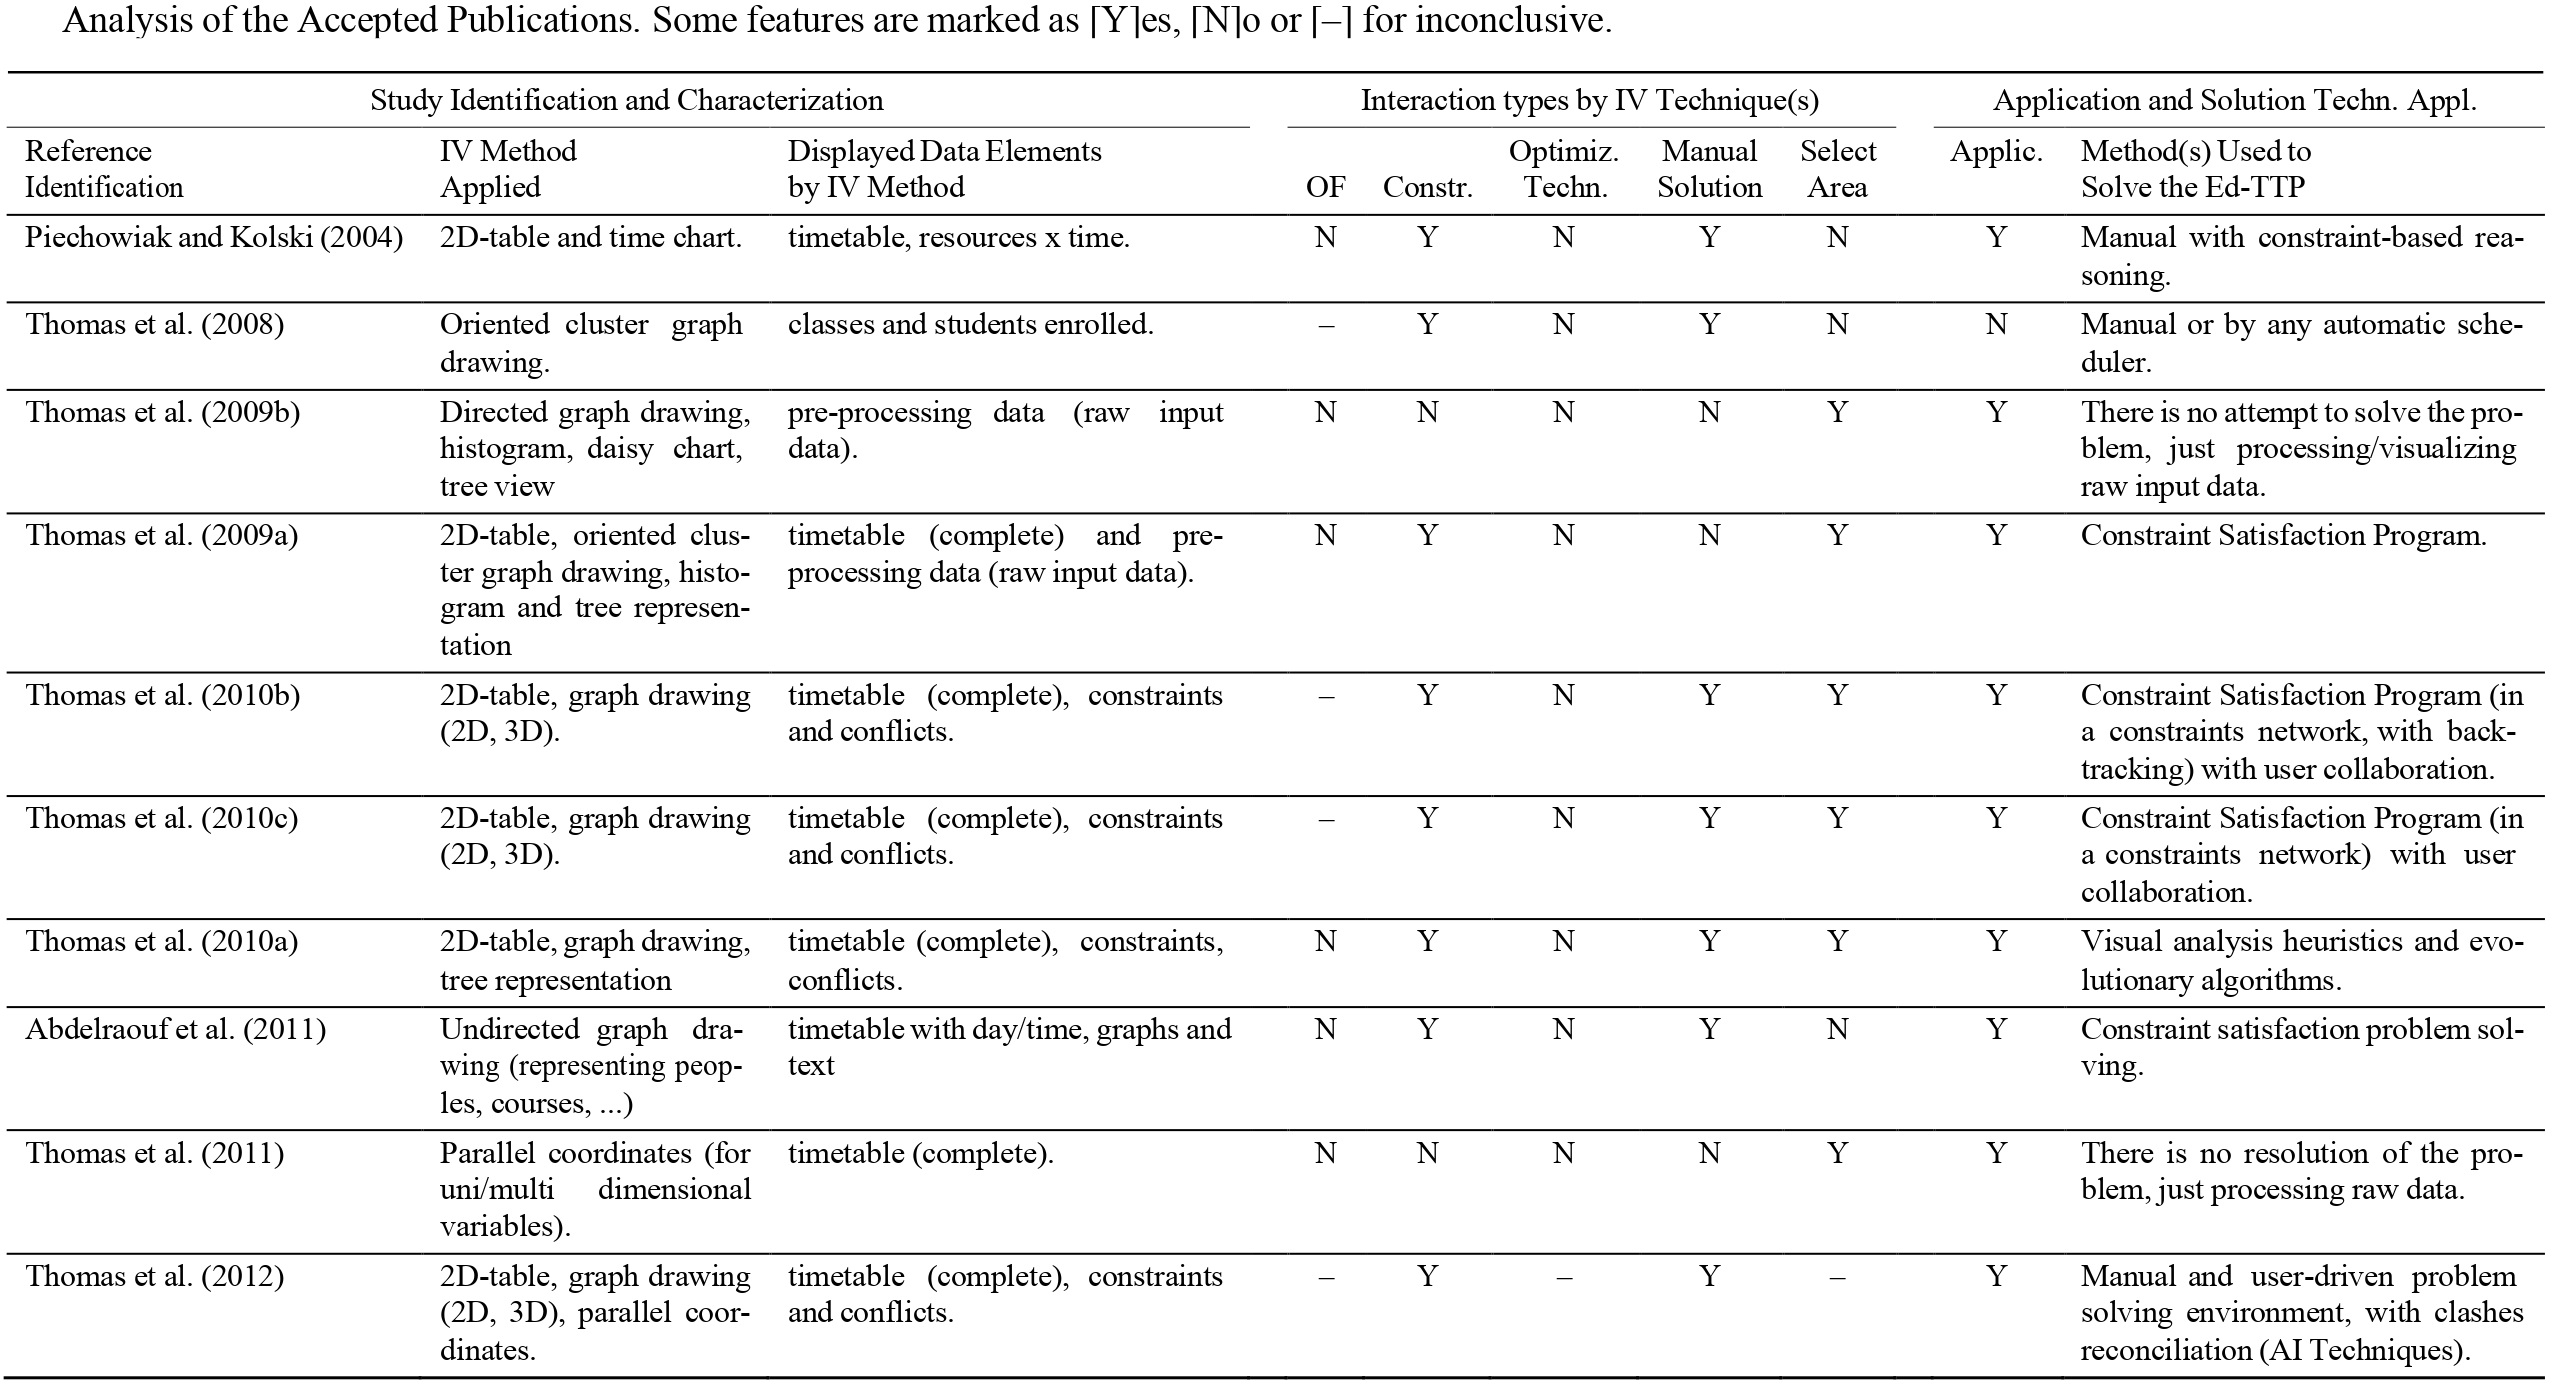
\includegraphics[angle=0,scale=0.7]{files/img/tabelas/Visualization.png}
    \legend{Fonte: \cite{alencar_visualization_2019} - editado}
\end{figure}    % Visualization

\section{Desafios recorrentes} % ### 2.3. Desafios recorrentes

Apesar da vasta quantidade de trabalhos realizados com este fim, o \textit{Timetabling Problem} segue sendo uma área sem uma solução definitiva.

Tomáš Müller \cite{burke_modeling_2007} traz a questão da modelagem como um dos maiores obstáculos. À medida em que a complexidade aumenta, se torna cada vez mais difícil desenvolver uma solução efetiva. Assim fazendo com que a solução para uma universidade possa não ter utilidade para outras, ou até mesmo não seja capaz de lidar com todos os problemas de uma mesma universidade.

Apesar do contrafluxo encontrado na resolução desse problema, Tomáš cita que, apesar da complexidade, é sim possível desenvolver soluções que tenham uso prático, mesmo que não seja um processo fácil. As ferramentas existem e estão disponíveis. Restando então considerar e resolver as preocupações dos usuários às questões, visto que as técnicas de resolução já se encontram vastamente documentados.

Com isso, entramos também no ramo da Interação Homem-Máquina, ramo abordado por Dinata \cite{andre_interaction_2018} que visou em seu desenvolvimento a criação de uma interface focada no usuário. Assim minimizando o atrito na abordagem desse problema complexo. Também sendo área de enfoque de \cite{alencar_visualization_2019} em sua revisão literária

% <!--
% ### 2.5. Contexto histórico e origem

% - Como surgiu essa área? Em que momento ela se dividiu? Devo falar sobre isso?

% ### 2.6. Técnicas existentes(?)

% - Falar sobre técnicas existentes e quem já fez. Tipo o que aquele artigo sem DOI fez
% -->

    \chapter{Modelagem geral do sistema}

Tendo esclarecido sobre as questões gerais do trabalho e da área de estudo. Agora nos aprofundaremos um pouco mais na modelagem e criação de diagramas que ilustrem o funcionamento geral do sistema e a forma como se dará a execução da metodologia proposta.

\section{Estágios de execução}

Em seu trabalho de aplicação prática, \cite{miranda_udpskeduler_2012} estruturou estágios que compõem o processo necessário para que enfim se alcance a definição de \textit{timetables} ótimas.

\begin{figure}[htbp]\centering
    \caption{\label{fig:geral} Estágios para a obtenção de grade horária ótima}
    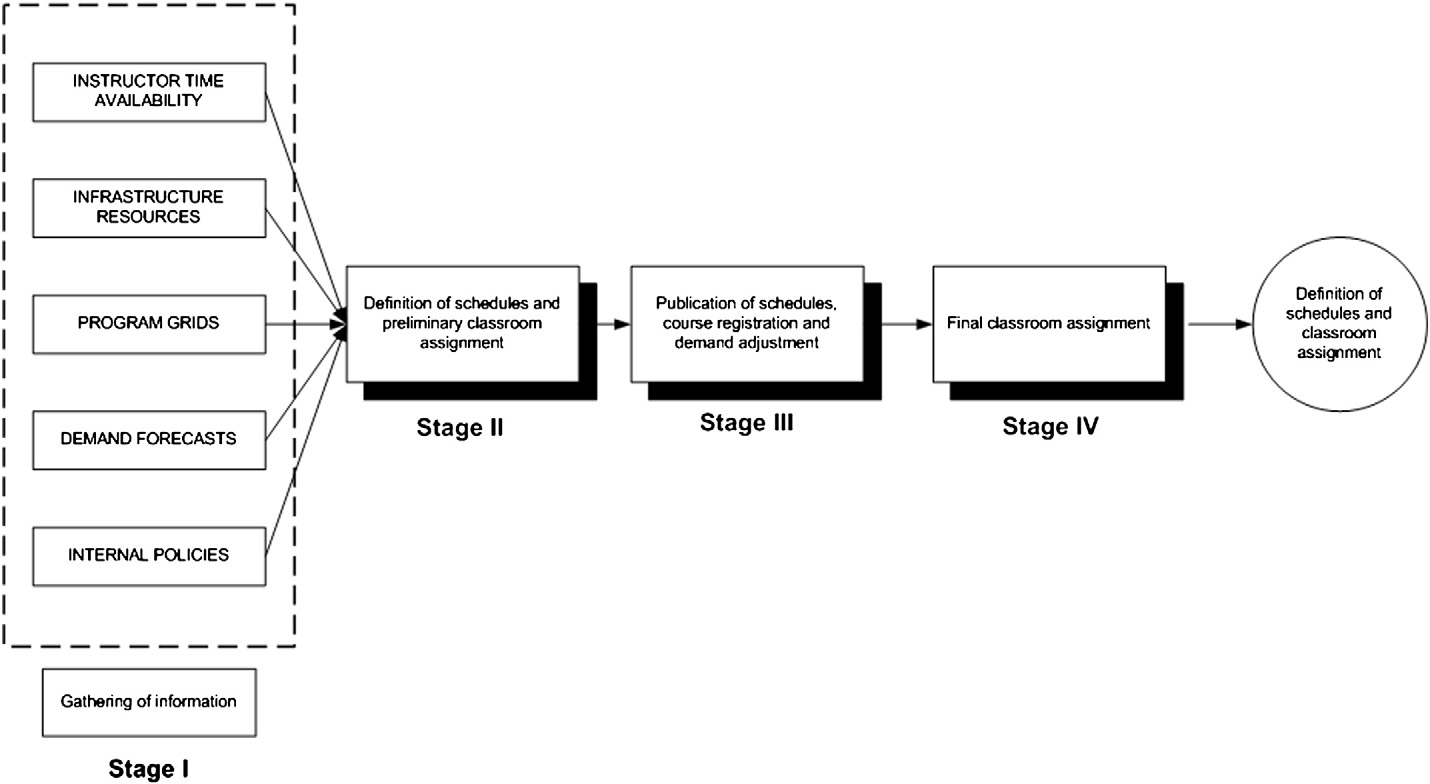
\includegraphics[scale=0.5]{files/img/Arquitetura/Arquitetura-UDP.png}
    \legend{Fonte: \cite{miranda_udpskeduler_2012}}
\end{figure}

Na Figura \ref{fig:geral}, estão dispostos 4 estágios principais. O primeiro dispõe da aquisição de informações. O meio de aquisição não é relevante para o momento atual, apenas considera-se que esta informação será obtida. No segundo estágios são definidas grades horárias preliminares para se atribuir os alunos. No terceiro, os alunos se inscrevem e a demanda é ajustada, por fim, no quarto estágio, ocorre a alocação final das salas.

\section{Iteração}

Para se alcançar uma alta satisfação por parte dos \textit{stakeholders}, vê-se necessária a constante interação com os mesmos. Para isto, será seguida a estrutura utilizada por \cite{andre_interaction_2018}.

\begin{figure}[htbp]\centering
    \caption{\label{fig:IxD} Etapas do Design de Interação}
    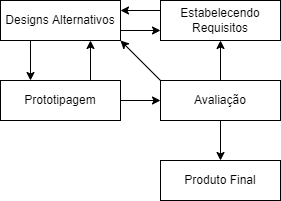
\includegraphics[scale=1]{files/img/Arquitetura/Arquitetura-IxD.png}
    \legend{Fonte: o autor}
\end{figure}    % University

Seguindo o conceito do Design de Interação, a Figura \ref{fig:IxD} ilustra o ciclo de ações a serem tomadas durante o desenvolvimento do sistema, caso este venha a ser necessário. Neste modelo de pesquisa, os \textit{stakeholders} serão consultados continuamente enquanto lhes é apresentado protótipos do sistema, para que assim informem quanto às suas percepções. Esta dinâmica tem como finalidade encontrar um design tal que seja adequado aos desejos e necessidades de seus usuários finais. 

\section{Funcionamento}

O sistema final seguirá uma dinâmica similar à que foi ilustrada por \cite{bebis_information_2019} em seu trabalho sobre o uso da Visualização de Informações em relação às Ed-TTPs.

\begin{figure}[htbp]\centering
    \caption{\label{fig:sistema} Funcionamento geral do sistema}
    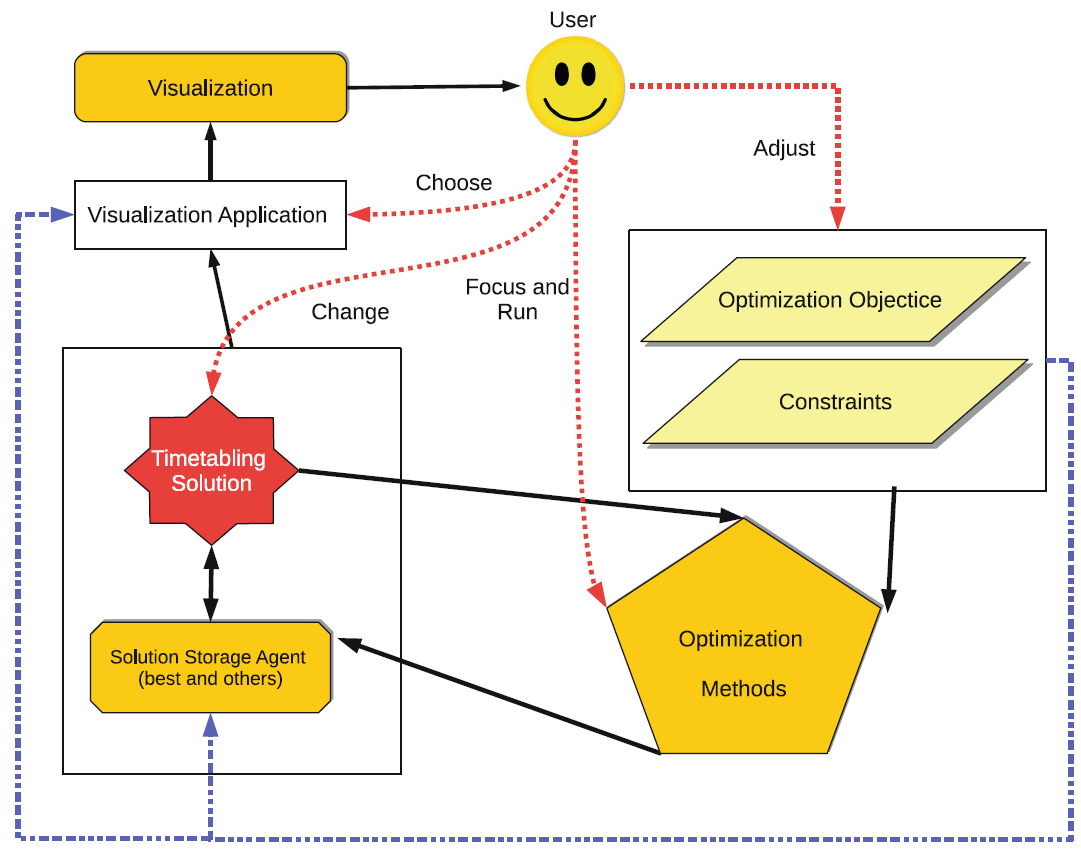
\includegraphics[scale=0.6]{files/img/Arquitetura/Arquitetura_bebis_information_2019.png}
    \legend{Fonte: \cite{bebis_information_2019}}
\end{figure}

A Figura \ref{fig:sistema} apresenta o comportamento geral do sistema, como seus diferentes segmentos interagem entre si e de que forma o usuário interage com o mesmo. O usuário poderá ajustar os objetivos da otimização e suas restrições, elas serão utilizadas nos métodos de otimização. Estes métodos serão utilizados para se alcançar soluções para estes critérios, as melhores serão então armazenadas. Em posso destes dados, a aplicação apresentará visualmente estas informações ao usuário, permitindo que ele interaja dinamicamente a fim de alcançar seus objetivos.

    
    % \chapter{Revisão da literatura}
    
    Alguns pontos relevantes a se aprofundar com a revisão literária são:
    
    \section{Qual é o problema?}
        
% [Usar a fonte para explicar o problema de timetabling: https://sci-hub.se/https://doi.org/10.1007/978-3-030-33720-9_21]
        O "problema de organização de grade horária" (\textit{timetabling problem}) é uma subcategoria do problema de \textbf{agendamento} (\textit{scheduling}) que por sua vez é definido por \cite{WREN1996} como sendo:

        \begin{quote}\footnotesize
            Resolver problemas práticos relacionados à alocação, sujeito a restrições, de recursos a objetos sendo colocados no espaço-tempo, usando ou desenvolvendo quaisquer ferramentas que possam ser apropriadas. Os problemas irão frequentemente se relacionar à satisfação de certos objetivos.
        \end{quote}
        
        Wren também informa que uma determinada \textit{timetable} apenas informa quando eventos serão realizados, e esse conceito se encaixa no que proponho neste documento. Entretanto, ele também diz que "a grade horária de classes de uma universidade deve levar em conta a disponibilidade de professores individualmente.", bem como a atribuição de salas, sendo ambos limitados por restrições duras e flexíveis (\textit{hard and soft constraints}).
    
    \section{Há solução?}
        
        Existem diversas implementações já realizadas, utilizando de uma variedade de métodos. Em seu trabalho, J. Miranda \cite{MIRANDA2012505} informa sobre diversos sistemas baseados em computador para auxiliar na tarefa de agendamento. J. Miranda também cita um dos métodos de resolução como sendo o \textbf{modelo de programação inteira} e \textbf{heurísticas}.
        
        % Já [Vinod](\ref{https://www.researchgate.net/publication/301564510_ACADEMIC_TIMETABLE_SCHEDULING_REVISITED}) cita diversos outros autores como: .[34](a) [64](a)D.Abramson(1991), D.Abramson et al (1999) proposed simulated annealing [66](a) [20](a) M. Wright(1996) used heuristic search and A. Schaerf (1999) used Local search techniques for School.
        
        % <!-- Preciso formatar muito direitinho isso daqui. Tem qualidade de referência, mas tá porco o uso -->
    
    \section{Quais são os desafios da solução do problema?}
        
        Também segundo J. Miranda, embora o problema de atribuição de salas não seja novo e tenha extensa literatura a seu respeito, são poucos os que de fato implementaram um sistema para suporte de decisões. Isso se dá por diversos fatores, também listado pelo autor fazendo referência a trabalhos anteriores, sendo alguns deles a resistência organizacional à mudanças e adoção de novas tecnologias, nível de dificuldade do problema, dentre outros.
        
        % <!-- Pegar a referência original? -->
        
        Outra característica é informada por Joshua \cite{THOMAS2009} que fala sobre a multidimensional do problema de timetabling. Por causa dessa questão há uma complexidade elevada para conseguir conceber visual e mentalmente de que forma os dados relacionados ao problema se estruturam, assim dificultando a elaboração de sistemas computacionais que auxiliem nessa tarefa.
        
        Tomáš Müller \cite{MURRAY2007} traz a questão da modelagem como um dos maiores obstáculos. À medida em que a complexidade aumenta, se torna cada vez mais difícil desenvolver uma solução efetiva. Assim fazendo com que a solução para uma universidade possa não ter utilidade para outras, ou até mesmo não seja capaz de lidar com todos os problemas de uma mesma universidade.
    
    \section{Como resolver os desafios?}
        
        Apesar do contra-fluxo encontrado na resolução dessa problema, Tomáš cita que, apesar da complexidade, é sim possível desenvolver soluções que tenham uso prático, mesmo que não seja um processo fácil. As ferramentas existem e estão disponíveis. Restando então considerar e resolver as preocupações dos usuários às questões além dos métodos de resolução.
        
        Com isso, entramos também no ramo da Interação Homem-Máquina, ramo abordado por Dinata \cite{ANDRE2018} que visou em seu desenvolvimento a criação de uma interface focada no usuário. Assim minimizando o atrito na abordagem desse problema complexo.

    % \chapter{Objetivos}

Como objetivos gerais, espera-se conseguir desenvolver um sistema de suporte à decisão tal que aumente a eficiência e eficácia do processo de criação de grades horárias que semestralmente demandam extensa quantidade de tempo dos coordenadores de curso na UENF. Nesse processo, também é esperado que as grades horárias finais tragam também benefícios aos alunos. Visto que estes muitas vezes lidam com grades horárias que não contemplam suas reais demandas.

Como objetivos mais específicos, podemos listar os seguintes:

\begin{enumerate}
    \item Entender de que forma os setores administrativos da UENF atualmente lidam com a questão do \textit{timetabling}
    \item Obter as demandas de aprimoramentos desejadas pelos diferentes centros e laboratórios
    \item Modelar o sistema de resolução de \textit{timetabling} de acordo com os requisitos demandados
    \item Encontrar o que é necessário para a adoção da aplicação de tabelamento de horário
    \item Incentivar o uso de uma ferramenta centralizada para a otimização do \textit{Timetabling Problem}
\end{enumerate}

    % \chapter{Metodologia}

Considerando as dificuldades encontradas em trabalhos anteriores, entende-se que o maior desafio será superar as especificidades que serão encontradas durante a modelagem da universidade em questão. Para isso, será inicialmente necessária uma pesquisa bibliográfica com foco no estudo das abordagens qualitativas realizadas anteriormente que obtiveram sucesso em elicitar os requisitos adequados para as instituições de ensino.

% <!-- Adicionar referência sobre pesquisa qualitativa? -->

Com este conhecimento, um material inicial para a pesquisa exploratória e qualitativa deve ser desenvolvido levando em conta as questões próprias da universidade em questão, visando também coletar dados relevantes para uma futura pesquisa com maior enfoque em características emergentes que a pesquisa anterior pode levantar.

Nesta primeira pesquisa, algumas informações esperadas revolvem em torno das percepções dos \textit{stakeholders} do sistema proposto, sendo esses principalmente os professores, coordenadores de cursos, chefes de laboratório e diretores de centro. Estas percepções incluem o entendimento deles quanto ao método atual e às alternativas existentes, nível de insatisfação com o método atual, nível de desejo quanto à um novo método, características e funcionalidades que gostariam de ter em um sistema de suporte à decisão. Solicitando também que deem informações adicionais que gostariam de acrescentar. Questionamentos similares também serão realizados com alunos, porém em formato de formulário online para facilitar o processamento dos dados coletados.

Tendo as informações dos \textit{stakeholders} primários em mãos, diagramas conceituais devem ser desenhados utilizando softwares de suporte como o \href{https://www.visual-paradigm.com/}{Visual Paradigm}, \href{drawio.com}{Draw.io} e/ou a \href{https://mermaid.js.org/}{ferramenta Mermaid}.

Munido destes dados, um sistema de suporte à decisão poderá ser desenvolvido para então ser usado como ferramenta centralizada, assim fazendo com que o objetivo geral seja alcançado.

    % \chapter{Cronograma das atividades} \label{atividades}

Cronograma de atividades ao longo dos meses de desenvolvimento do trabalho

\begin{table}[H]
    \centering
    \resizebox{\textwidth}{!}{%
    \begin{tabular}{@{}l|l|l|l|l|l|l|l|l|@{}}
    \toprule

    \multicolumn{1}{c|}{\textbf{Atividades}} &
    \multicolumn{1}{c|}{\textbf{Maio}} &
    \multicolumn{1}{c|}{\textbf{Junho}} &
    \multicolumn{1}{c|}{\textbf{Julho}} &
    \multicolumn{1}{c|}{\textbf{Agosto}} &
    \multicolumn{1}{c|}{\textbf{Setembro}} &
    \multicolumn{1}{c|}{\textbf{Outubro}} &
    \multicolumn{1}{c|}{\textbf{Novembro}} &
    \multicolumn{1}{c|}{\textbf{Dezembro}} \\ \midrule
    
    
    \multicolumn{1}{|l|}{\textbf{Pesquisa bibliográfica}}               & \cellcolor[HTML]{A4C2F4} & \cellcolor[HTML]{A4C2F4} & \cellcolor[HTML]{A4C2F4} & & & & & \\ \midrule
    \multicolumn{1}{|l|}{\textbf{Desenvolvimento do sistema}}           & \cellcolor[HTML]{A4C2F4} & \cellcolor[HTML]{A4C2F4} & \cellcolor[HTML]{A4C2F4} & \cellcolor[HTML]{A4C2F4} & \cellcolor[HTML]{A4C2F4} & \cellcolor[HTML]{A4C2F4} & \cellcolor[HTML]{A4C2F4} & \\ \midrule
    \multicolumn{1}{|l|}{\textbf{Pesquisa exploratória qualitativa}}    & & \cellcolor[HTML]{A4C2F4} & \cellcolor[HTML]{A4C2F4} & \cellcolor[HTML]{A4C2F4} & & & & \\ \midrule
    \multicolumn{1}{|l|}{\textbf{Obtenção de requisitos}}               & & \cellcolor[HTML]{A4C2F4} & \cellcolor[HTML]{A4C2F4} & \cellcolor[HTML]{A4C2F4} & & & & \\ \midrule
    \multicolumn{1}{|l|}{\textbf{Validação do sistema desenvolvido}}    & & & \cellcolor[HTML]{A4C2F4} & \cellcolor[HTML]{A4C2F4} & \cellcolor[HTML]{A4C2F4} & \cellcolor[HTML]{A4C2F4} & \cellcolor[HTML]{A4C2F4} & \\ \midrule
    \multicolumn{1}{|l|}{\textbf{Escrita final do documento}}           & & & & & & & \cellcolor[HTML]{A4C2F4} & \cellcolor[HTML]{A4C2F4} \\ \midrule
    \multicolumn{1}{|l|}{\textbf{Apresentação}}                         & & & & & & & & \cellcolor[HTML]{A4C2F4} \\ \midrule
    \multicolumn{1}{|l|}{\textbf{Apresentação}}                         & & & & & & & & \cellcolor[HTML]{A4C2F4} \\ \bottomrule
    
    \end{tabular}%
    }
    \caption{Etapas do Projeto de Pesquisa}
    \label{tab:etapas}
\end{table}
    
    % % --- PARTE --- %
\part{Referenciais teóricos}

% --- Capitulo de revisão de literatura --- % % NÃO USADO
    % % --- PARTE --- %
\part{Resultados}

% --- primeiro capitulo de Resultados --- %

% --- segundo capitulo de Resultados --- %
            % NÃO USADO
    % \chapter{Conclusão}             % --- CONCLUSÃO --- % NÃO USADO
    
\postextual                                     % --- INÍCIO DOS ELEMENTOS PÓS-TEXTUAIS --- %

    \bibliography{files/referencias}      % --- Referências bibliográficas --- %
    % \glossary                                 % --- Glossário --- % NÃO USADO
    % % ---
\begin{apendicesenv}

% Imprime uma página indicando o início dos apêndices
\partapendices



% ----------------------------------------------------------
%\chapter{Quisque libero justo}
% ----------------------------------------------------------

\lipsum[50]

% ----------------------------------------------------------
\chapter{Nullam elementum urna vel imperdiet sodales elit ipsum pharetra ligula
ac pretium ante justo a nulla curabitur tristique arcu eu metus}
% ----------------------------------------------------------
\lipsum[55-57]

\end{apendicesenv}
% ---


% ----------------------------------------------------------
% Anexos
% ----------------------------------------------------------

% ---
% Inicia os anexos
% ---
\begin{anexosenv}

% Imprime uma página indicando o início dos anexos
\partanexos

% ---
%\chapter{Morbi ultrices rutrum lorem.}
% ---
\lipsum[30]

% ---
%\chapter{Cras non urna sed feugiat cum sociis natoque penatibus et magnis dis
%parturient montes nascetur ridiculus mus}
% ---

\lipsum[31]

% ---
%\chapter{Fusce facilisis lacinia dui}
% ---

\lipsum[32]

\end{anexosenv}
             % --- Inicia os apêndices --- % NÃO USADO
    % \phantompart
\printindex      % --- INDICE REMISSIVO --- %

\end{document}
